\chapter{Motivacional}
\section{Introducción}
Se han definido una serie de puntos de vista estándar para modelar los aspectos motivadores. Cada uno de estos puntos de vista presenta una perspectiva diferente para modelar la motivación que subyace en algunas arquitecturas empresariales y permite al modelador centrarse en ciertos aspectos. Por lo tanto, cada punto de vista considera sólo una selección de los elementos y relaciones que se han descrito en el capítulo 3.

Se distinguen los siguientes puntos de vista:

\begin{itemize}
	\item El punto de vista de los interesados se centra en la elaboración de modelos de los interesados, los factores determinantes, las evaluaciones de esos factores y los objetivos iniciales para abordar esos factores y evaluaciones.
	\item El punto de vista de la realización de los objetivos se centra en el perfeccionamiento de los objetivos iniciales de alto nivel para convertirlos en (sub)objetivos más concretos mediante la relación de agregación y, por último, en requisitos y limitaciones mediante la relación de realización.
	\item El punto de vista de la contribución al logro de objetivos se centra en la modelización y el análisis de las relaciones de influencia entre los objetivos (y los requisitos).
	\item El punto de vista de los principios se centra en la modelización de los principios pertinentes y las metas que motivan esos principios.
	\item El punto de vista de la realización de los requisitos se centra en la modelización de la realización de los requisitos y las limitaciones por medio de elementos básicos, como los agentes, los servicios, los procesos, los componentes de la aplicación, etc.
	\item El punto de vista de la motivación abarca todo el aspecto de la motivación y permite utilizar todos los elementos de motivación.
\end{itemize}

A continuación se describen por separado todos los puntos de vista. Para cada punto de vista, se indican sus elementos y relaciones, las directrices para su utilización, su objetivo y grupo destinatario. Además, la descripción de cada punto de vista contiene modelos de casos.
\newpage

\section{Metamodelo}
\begin{figure}[h!]
	\centering
	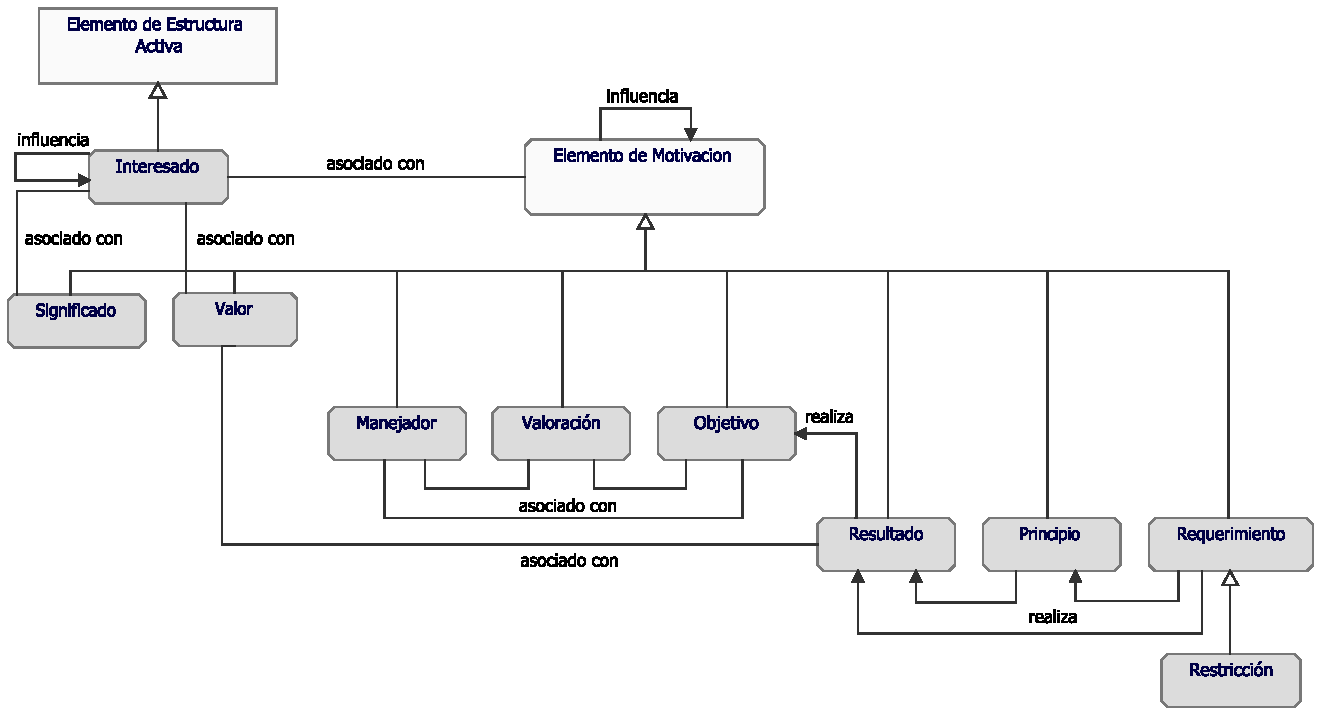
\includegraphics[width=1.0\linewidth]{imgs/meta/Motivacion}
	\caption{Metamodelo Motivacional}
\end{figure}

La principal jerarquía de los elementos de comportamiento y estructura del lenguaje ArchiMate se presenta en el metamodelo de la Figura 4.1. Define estos elementos de manera genérica e independiente de la capa. Observe que la mayoría de estos elementos (las cajas blancas) son elementos abstractos del meta modelo; es decir, no están instanciados en los modelos sino que sólo sirven para estructurar el meta modelo.  La notación presentada en este capítulo es, por lo tanto, la forma genérica en que se representan las especializaciones de estos elementos (es decir, los elementos de las diferentes capas de la arquitectura).  Los elementos concretos (las cajas grises), que pueden ser utilizados para modelar la Arquitectura de la Empresa a un nivel estratégico.\\ \\

Este fragmento genérico de metamodelo consiste en dos tipos principales de elementos: elementos de estructura ('sustantivos') y elementos de comportamiento ('verbos').

\newpage
\section{Punto de Vista de Implicados}
El punto de vista de las partes interesadas permite al analista modelar las partes interesadas, los impulsores internos y externos del cambio y las evaluaciones (en términos de fortalezas, debilidades, oportunidades y amenazas) de estos impulsores. También se pueden describir los vínculos con los objetivos iniciales (de alto nivel) que abordan estas preocupaciones y evaluaciones. Estas metas forman la base del proceso de ingeniería de requisitos, incluyendo el refinamiento de las metas, el análisis de la contribución y el conflicto, y la derivación de los requisitos que realizan las metas.

\subsection{Modelo de Implicados}
\begin{figure}[h!]
	\centering
	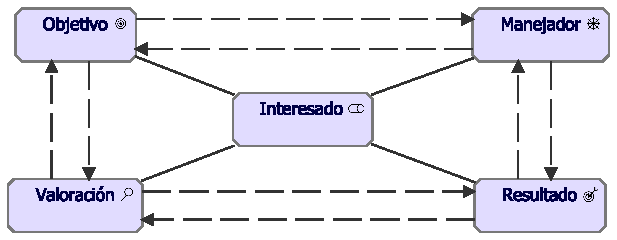
\includegraphics[width=1.0\linewidth]{imgs/modelo/Interesado}
	\caption{Modelo Implicados}
\end{figure}

Los elementos de motivación se utilizan para modelar las motivaciones, o razones, que guían el diseño o el cambio de una arquitectura empresarial, y es esencial comprender los factores, a menudo denominados impulsores, que influyen en otros elementos de motivación.  Pueden originarse tanto dentro como fuera de la empresa.  Los impulsores internos, también llamados preocupaciones, están asociados con las partes interesadas, que pueden ser algún ser humano individual o algún grupo de seres humanos, como un equipo de proyecto, una empresa o la sociedad. Ejemplos de esos impulsores internos son la satisfacción del cliente, el cumplimiento de la legislación o la rentabilidad. Es común que las empresas realicen una evaluación de esos factores impulsores; por ejemplo, utilizando un análisis FODA, a fin de responder de la mejor manera posible.

%\newpage

\subsection{Caso  de Implicados}
\begin{figure}[h!]
	\centering
	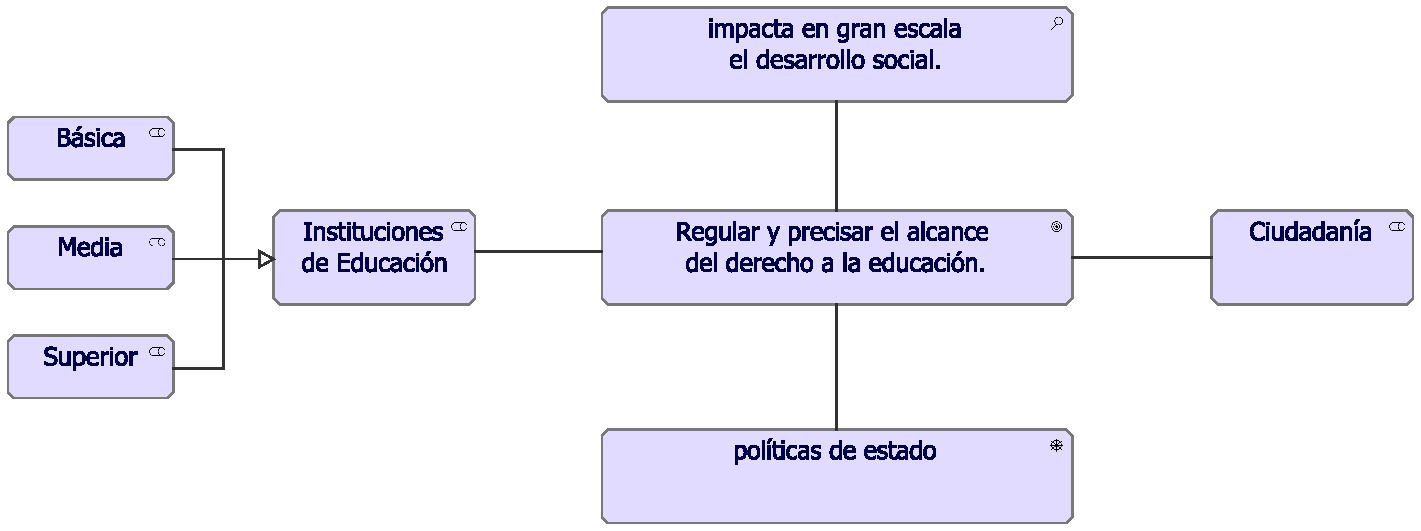
\includegraphics[width=1.0\linewidth]{imgs/motivacion/implicados/imp1.pdf}
	\caption{Caso Implicados}
\end{figure}

Los elementos, principalmente externos que se encuentran fuertemente ligados para regular y precisar el alcance del derecho a la educación, son las políticas de Estado vigentes y en desarrollo dispuestas por la administración a cargo. Por otra parte, la valoración comprendida en este objetivo, impacta en gran medida el desarrollo social del país, debido a que son ellos, la comunidad quienes dispondrán de la oportunidad educarse para forjar un mejor futuro tanto para sus familias como para la comunidad en general. Así mismo, las instituciones de educación básica, media y superior, quienes permiten y promueven la adquisición de habilidades, conocimientos y la ampliación de horizontes personales, a través de los lineamientos dispuestos por el MEN, son otro de los interesados alrededor de este objetivo.
\section{Punto de Vista de la Realización de Objetivos}

El punto de vista de la realización de objetivos permite a un diseñador modelar el refinamiento de los objetivos (de alto nivel) en objetivos más tangibles, y el refinamiento de los objetivos tangibles en requisitos o restricciones que describen las propiedades que se necesitan para realizar los objetivos. El refinamiento de los objetivos en subobjetivos se modela utilizando la relación de agregación. El refinamiento de los objetivos en requisitos se modela utilizando la relación de realización.
Además, se pueden modelar los principios que guían el refinamiento de las metas en requisitos.

\subsection{Modelo de la Realización de Objetivos}
\begin{figure}[h!]
	\centering
	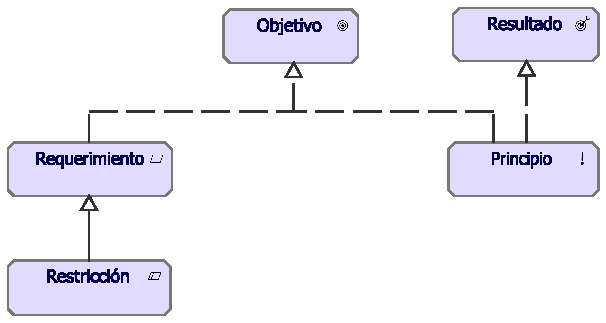
\includegraphics[width=1.0\linewidth]{imgs/modelo/RealObjetivos.pdf}
	\caption{Modelo Realización de Objetivos}
\end{figure}

La motivación de una organización o persona para lograr ciertos resultados está representada por las metas, los principios, los requisitos y las limitaciones. Las metas representan que un interesado quiere lograr un determinado resultado; por ejemplo, "Aumentar la satisfacción del cliente en un 10\%". Los resultados finales obtenidos por las capacidades que realizan estas metas son los resultados.

Un objetivo representa una declaración de intenciones de alto nivel, una dirección o un estado final deseado para una organización y sus partes interesadas.

\newpage

\subsection{Caso de la Realización de Objetivos}
\begin{figure}[h!]
	\centering
	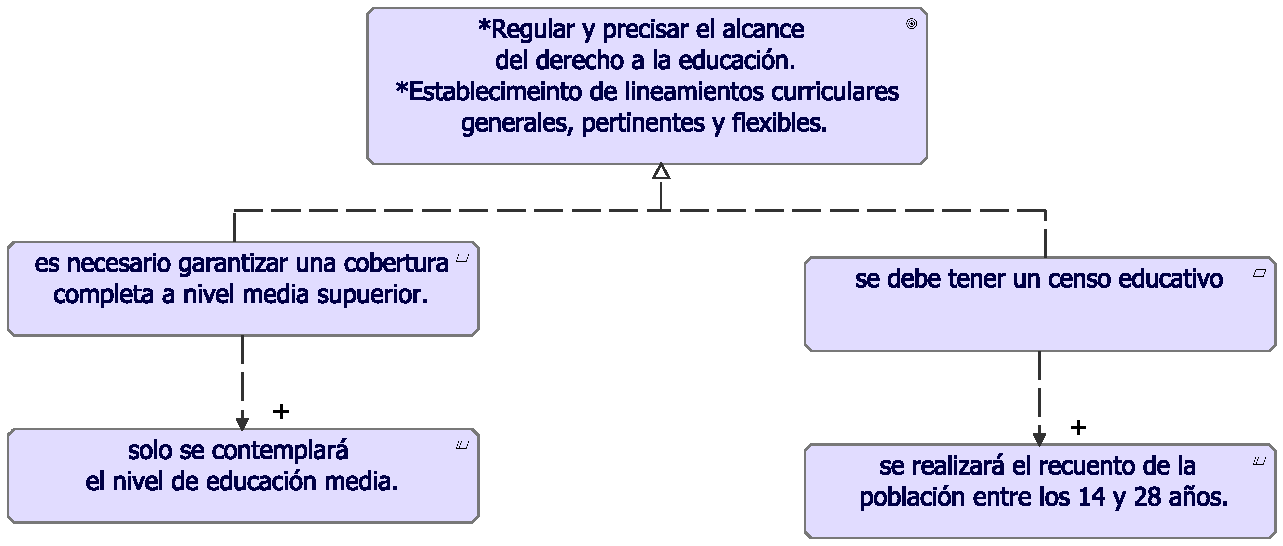
\includegraphics[width=1.0\linewidth]{imgs/motivacion/realizacionObj/realizacion.pdf}
	\caption{Caso Realización de Objetivos}
\end{figure}

Los requerimientos necesarios para regular y precisar el alcance del derecho a la educación, así como para dar alcance al objetivo de establecer los lineamientos curriculares, generales, pertinentes y flexibles radican en garantizar una cobertura completa en la educación media superior del país, que permita abrir una brecha para la implantación de esta ofertas educativas con aras de que logren mantenerse y adquirir una mayor demanda a través de las regulaciones del MEN para dar alcance al derecho de la educación a toda la comunidad. Igualmente, otro requerimiento indispensable para la consecución de estos objetivos planteados, es la realización de un censo educativo que proporcione un conocimiento certero sobre las características de la población a la cual está dirigida esta política inclusiva de educación y que además, provea de información vitalicia para la construcción y/o adecuación de las ofertas educativas de lineamientos curriculares generales, flexibles, pertinentes y flexibles. \\ \\
No obstante, una limitación en el requerimiento dispuesto para la garantía de una cobertura completa a nivel media superior es que, solo se contemplará la identificación vocacional en la transición de un nivel de educación media a superior, postergando la identificación vocacional a través de la gamificación en la transición de educación básica a educación media. A causa de este limitante, el censo educativo, aunque se realizará de forma general, en su etapa posterior del proceso, solo se hará énfasis en el recuento de la población entre los 14 y 28 años.
\section{Punto de Vista de Contribución de Objetivos}
Contribución de objetivos es uno de los puntos de vista de la parte motivacional, este punto de vista permite profundizar y ahondar en los objetivos planteados en el proyecto, con el fin de precisar y aclarar las metas propuestas por medio de una especie de desglose de información. Esta contribución de objetivos como su nombre lo indica, no es única y exclusivamente de un solo objetivo, sino que por el contrario, dependiendo del caso y si hay objetivos relacionados entre si, se pueden agrupar en un solo paquete de objetivo para realizar esta contribución de una manera más personalizada y completa, procurando en todo momento la optimización de todos los recursos.

\subsection{Modelo de Contribución de Objetivos}
\begin{figure}[h!]
	\centering
	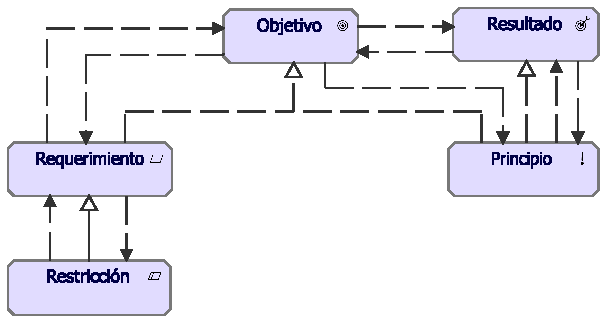
\includegraphics[width=1.0\linewidth]{imgs/modelo/ContObjetivos}
	\caption{Modelo Contribución de objetivos}
\end{figure}

El punto de vista de contribución de objetivos, presenta un modelo el cual como su nombre lo indica, se centra en un objetivo del proyecto planteado, del cual se desglosan ciertos requerimientos para este objetivo según sea el caso, sin dejar de mencionar que estos requerimientos pueden presentar en alguna ocasiones ciertas restricciones que son de vital importancia aclarar y mencionar para tener en cuenta en la estructuración del proyecto. Además de esto, siempre en cada modelo se busca un resultado o un fin específico, con este terminaría el punto de vista de contribución de objetivos.

%\newpage

\subsection{Caso  de Contribución de Objetivos}
\begin{figure}[h!]
	\centering
	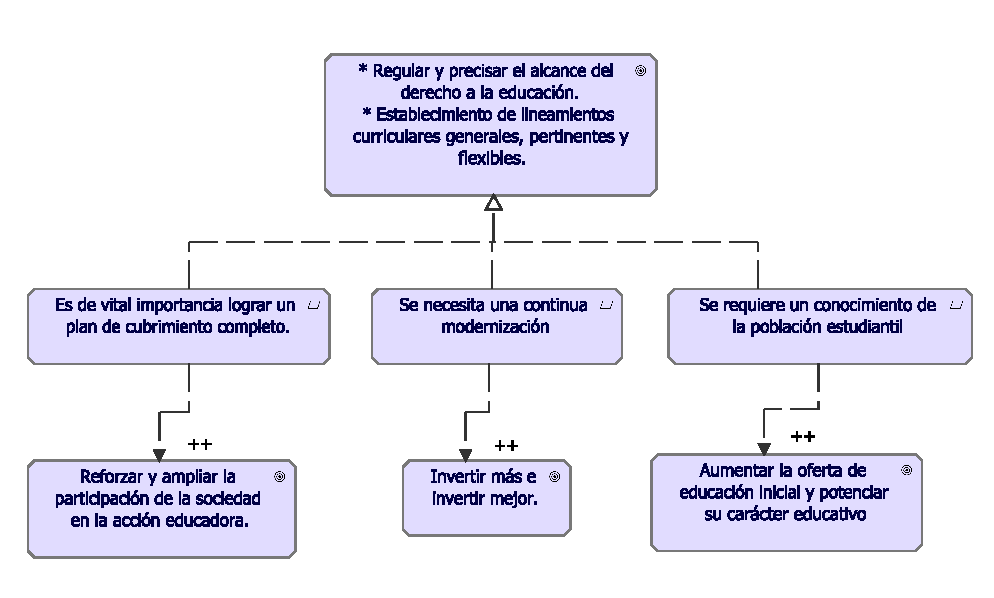
\includegraphics[width=1.0\linewidth]{imgs/motivacion/contriObjetivos/contriObjetivos.pdf}
	\caption{Caso Contribución de Objetivos}
\end{figure}

En el caso del proyecto planteado, en la sección de objetivos se postularon dos de estos, los cuales son transversales y están estrechamente relacionados, lo cual permite que se puedan trabajar al unisono, estos objetivos son: regular y precisar el alcance del derecho a la educación y establecimiento de lineamientos curriculares generales, pertinentes y flexibles. Ademas de esto, se plantearon tres requerimientos para estos objetivos, el primero de estos requerimientos se refiere a la importancia de lograr un plan de cubrimiento completo en educación para así cumplir con el objetivo de regular y precisar el alcance del derecho a la educación, el segundo requerimiento hace referencia a la modernización continua en la educación, para lo que se necesita más y mejor educación y finalmente, se encuentra el tercer requerimiento el cual indica la necesidad de un conocimiento de la población estudiantil con el fin de aumentar la oferta de educación inicial y potenciar su carácter educativo. De esta manera se realiza el punto de vista de contribución de objetivos, teniendo en cuenta los requerimientos a estos objetivos.

\section{Punto de Vista de Principios}
El punto de vista de principios permite al arquitecto crear una descripción detallada de los principios relacionados con un objetivo ou objetivos específicos de la organización, con el fin de proyectar los valores que propulsan el desarrollo de estos objetivos estratégicos.

\subsection{Modelo de Principios}
\begin{figure}[h]
	\centering
	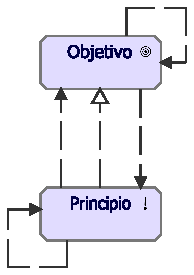
\includegraphics[width=0.3\linewidth]{imgs/modelo/Principios}
	\caption{Modelo Principios}
\end{figure}

Los elementos del modelo de principios permiten transmitir la relación univoca o biunívoca que hay entre los principios de la organización o empresa y los objetivos de la misma. Es una guía del diseño arquitectural de los principios corporativos que se aplican al prestar los servicios de la empresa por medio de valoraciones. Un principio representa una declaración cualitativa de intenciones que la arquitectura debe cumplir.

%\newpage

\subsection{Caso  de Principios}
\begin{figure}[h]
	\centering
	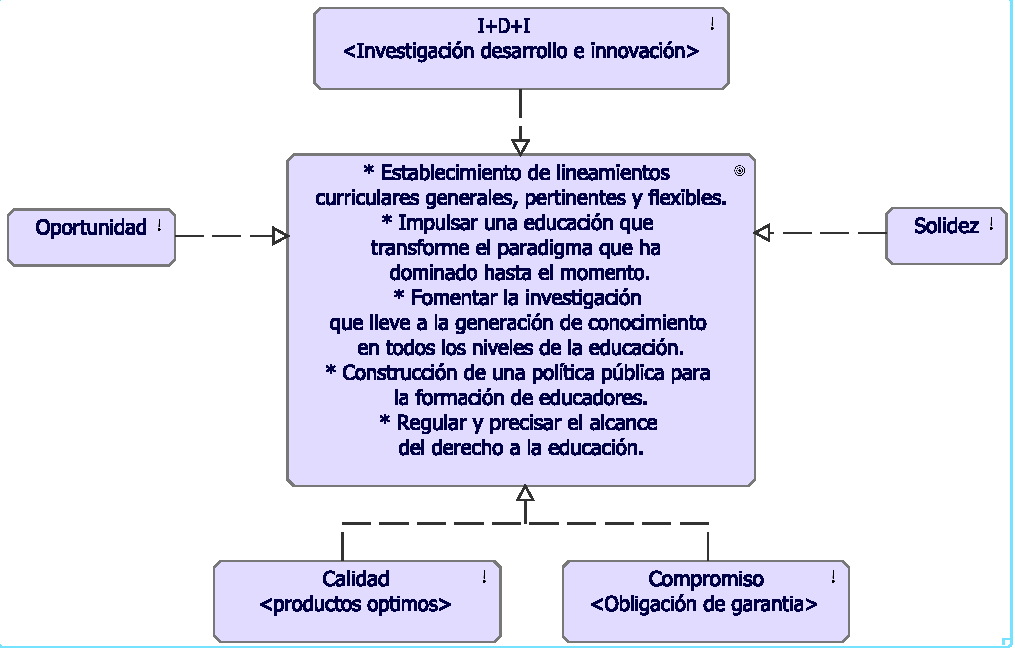
\includegraphics[width=1.0\linewidth]{imgs/motivacion/principios/principios}
	\caption{Caso Principios}
\end{figure}

Los principios que cualifican los objetivos corporativos relacionados con la calidad de la educación son aquellos que permiten el avance de forma asertada de lo que tiene que ver con el enfoque del fomento de investigaciones e impulso a la educación a un nivel mas alto, entre ellos tenemos la investigación desarrollo e innovación, calidad y compromiso.

%\newpage

\subsection{Caso  de Principios}
\begin{figure}[h]
	\centering
	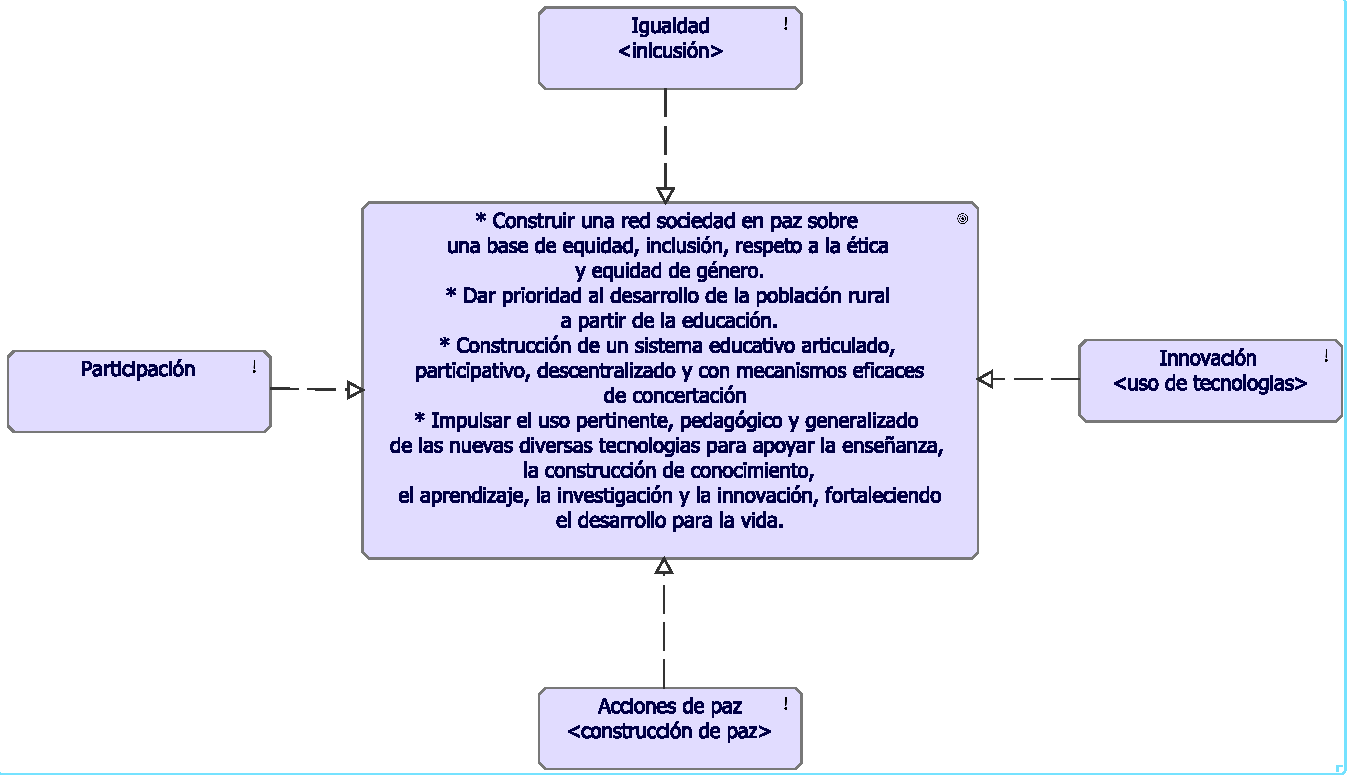
\includegraphics[width=1.0\linewidth]{imgs/motivacion/principios/principios_2}
	\caption{Caso Principios}
\end{figure}

Para construir la paz en nuestro país por medio de la educación que propone el MEN, se logra por medio de los principios que son base esencial para encontrar un equilibrio en la sociedad que potencie la entidad humana como se presentan en ek punto de vista de principios, entre ellos se tiene igualdad, participación, acciones de paz e innovación.
\section{Punto de Vista de Realización de Requerimientos}
El punto de vista de realización de requerimientos se basa en las necesidades que se requieren subsanar y que el sistema debe cumplir de manera satisfactoria, estos requerimientos, son los que definen las funciones que el sistema será capaz de realizar, describiendo las transformaciones que el sistema realiza sobre las entradas para producir salidas. Por decirlo de otra manera, estos requerimientos son los que posteriormente se van a transformar en algoritmos, es decir, en las funcionalidades del sistema.
Para la obtención de estos requerimientos, es necesario ademas de cumplir a detalle con una serie de pasos específicos, tener los objetivos, los cuales son el punto de partida para los requerimientos. Esta serie de pasos son: obtención, análisis, especificación, verificación y aceptación. Luego de esto, en la realización de requerimientos es en donde se especializan estos requerimientos.


\subsection{Modelo de Realización de Requerimientos}
\begin{figure}[h!]
	\centering
	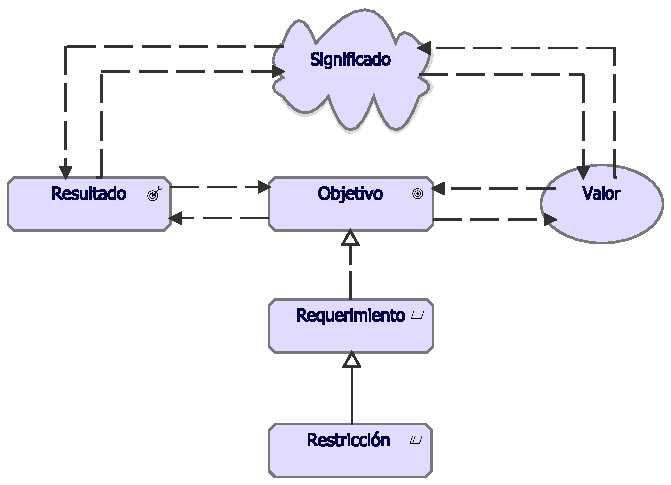
\includegraphics[width=1.0\linewidth]{imgs/modelo/RealRequerimientos}
	\caption{Modelo Realización de Requerimientos}
\end{figure}

El modelo del punto de vista de realización de requerimientos, como se ha evidenciado en los anteriores puntos de vista, parte de un objetivo central, del cual todo se desglosa, cuenta con diversas partes y herramientas como lo es el significado, valor, resultado y finalmente un requerimiento el cual se puede especializar cuantas veces lo permita.

%\newpage

\subsection{Caso  de Contribución de Objetivos}
\begin{figure}[h!]
	\centering
	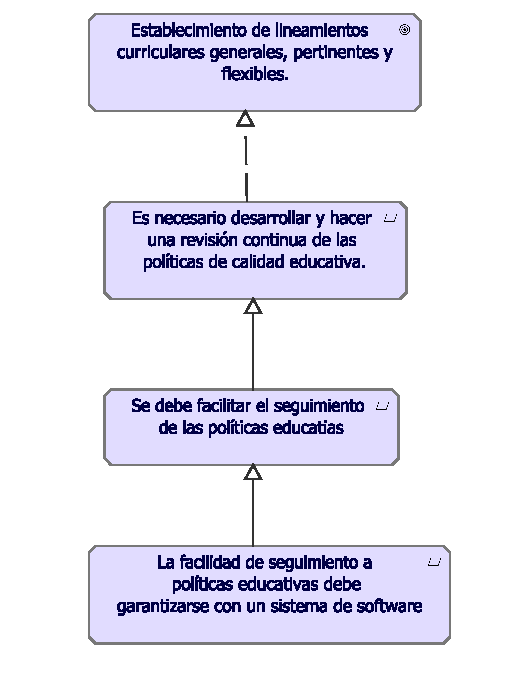
\includegraphics[width=0.6\linewidth]{imgs/motivacion/RealizaRequerimientos/realizaRequerimientos.pdf}
	\caption{Caso Realización de Requerimientos}
\end{figure}

En el proyecto planteado con el ministerio de educación nacional (MEN), y para la construcción del punto de vista de realización de requerimientos, en primer lugar se escogió un objetivo central del proyecto el cual es, Establecimiento de lineamientos curriculares generales, pertinentes y flexibles. A partir de este objetivo central, se dedujo un requerimiento como lo es: es necesario desarrollar y hacer una revisión continua de las políticas de calidad educativa, requerimiento del cual se puede especializar, tal como se hizo con el proyecto: se debe facilitar el seguimiento de las políticas educativas, y a su vez, esta especialización de requerimiento se pudo especializar una vez más: la facilidad de seguimiento a políticas educativas debe garantizarse con un sistema de software. Esta especialización de los requerimientos en la realización de los mismos, se puede hacer tantas veces como el mismo requerimiento lo permita.
\section{Punto de Vista de Motivación}
En esta vista de motivación permite diseñar al modelador los elementos de motivación por medio de influenciadores. En esta vista se resume las vistas anteriores dando lugar a tener las caracterizaras mas importantes de la vista motivacional.

\subsection{Modelo de Motivación}
\begin{figure}[h!]
	\centering
	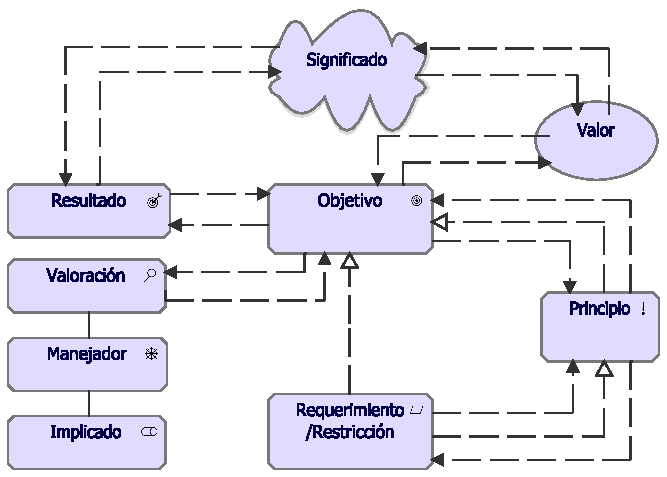
\includegraphics[width=1.0\linewidth]{imgs/modelo/Motivacion}
	\caption{Modelo Motivación}
\end{figure}

Los elementos de motivación se utilizan para modelar las motivaciones, o razones, que guían el diseño o cambio de una arquitectura empresarial. Entre los elementos mas importantes se tiene el implicado: aquel que se implica en el objetivo estudiado, por otro lado tenemos el alcance: aquel que da la motivación, entre otros mas elementos que radican en la motivación e influencia que ejercen sobre los objetivos estratégicos

%\newpage

\subsection{Caso  de Motivación}
\begin{figure}[h!]
	\centering
	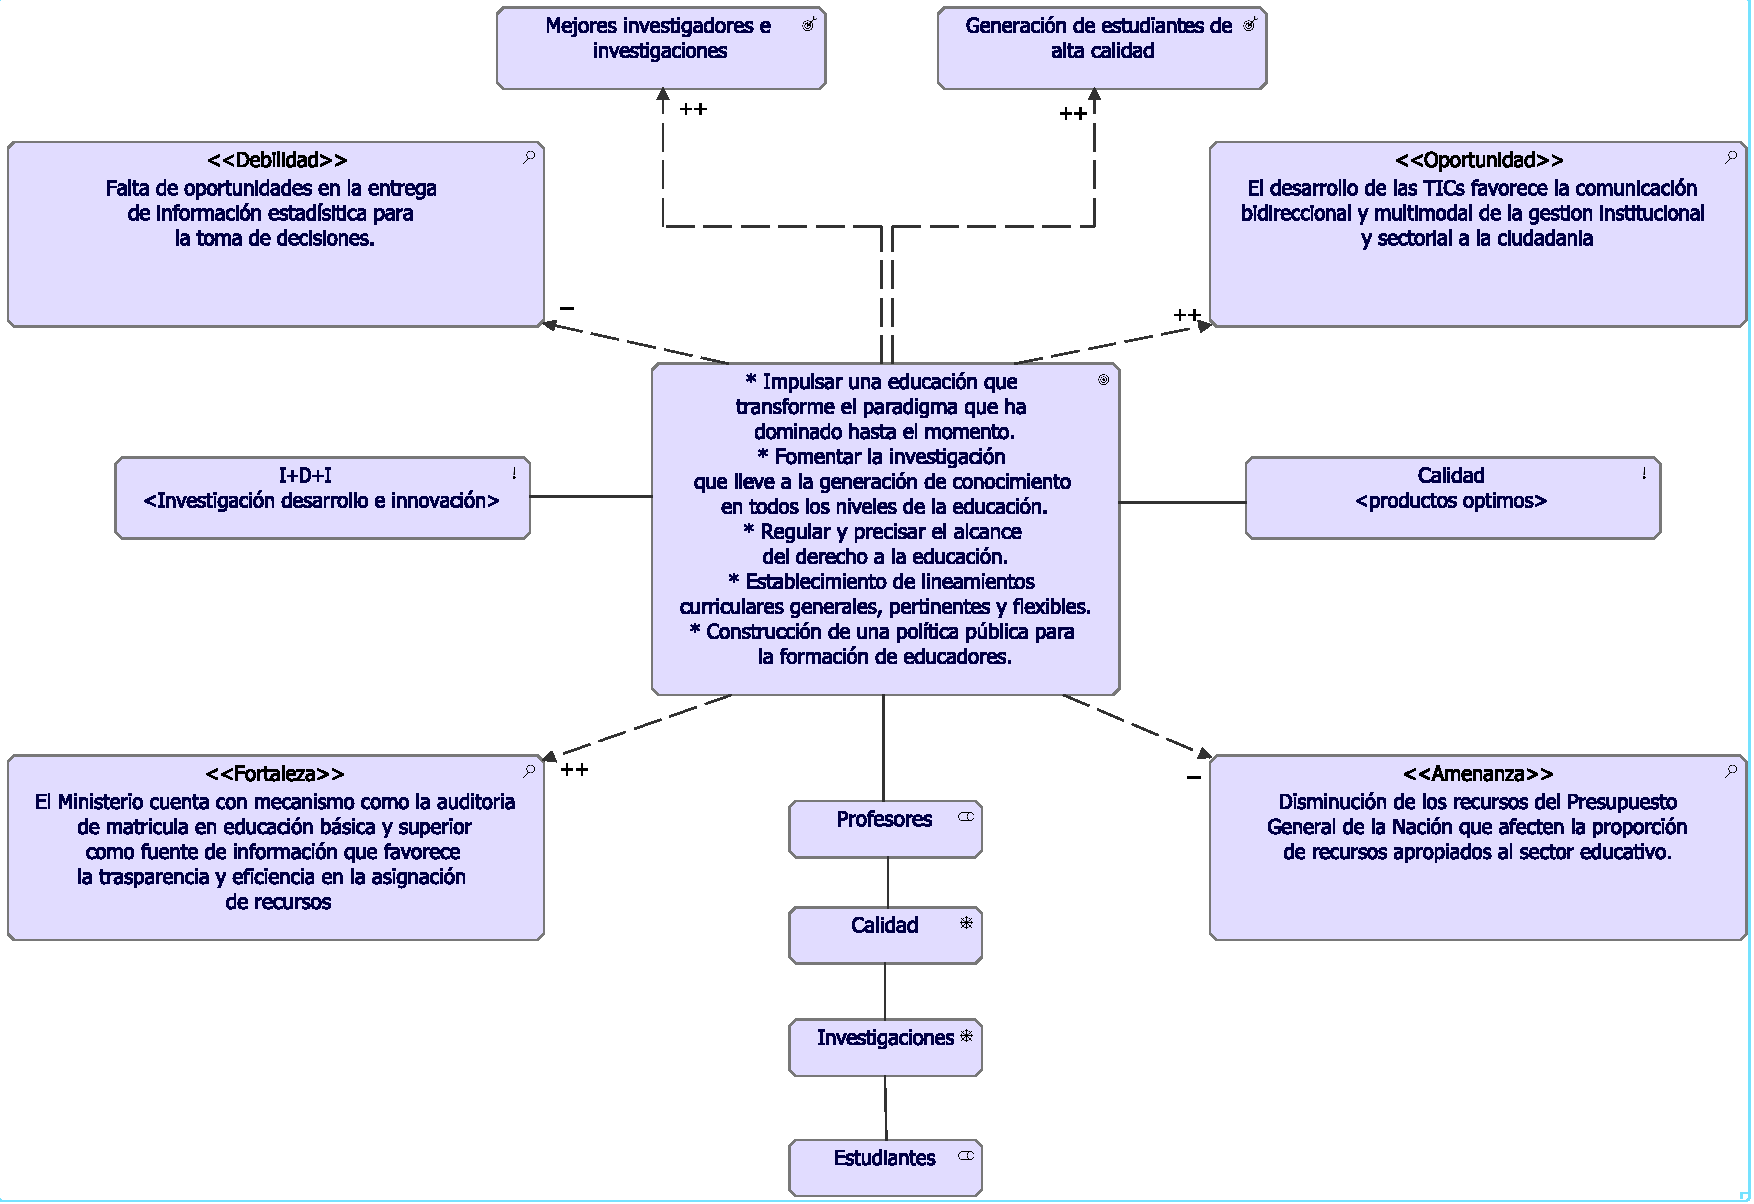
\includegraphics[width=1.0\linewidth]{imgs/motivacion/motivacion/motivacion}
	\caption{Caso Motivación}
\end{figure}

El análisis DOFA es un importante elemento que permite encontrar las estrategias que envuelven objetivos con el fin de mejorar los fines de una empresa. Para los objetivos agrupados en el caso de estudio de motivación tenemos las fortaleza: el ministerio usa la auditoria de la educación para favorecer la eficiencia de los recursos suministrados. La falta de oportunidad para tomar decisiones es una debilidad de la organización. Los implicados que están relacionados con una educación de calidad en este caso de estudio se tienen a los profesores impulsando calidad en sus enseñanzas logrando investigaciones y estudiantes de tal grado.    



